\documentclass{article}
\usepackage[utf8]{inputenc}
\usepackage{listings}
\usepackage{hyperref}
\usepackage{amsmath}
\usepackage{amssymb}
\usepackage{graphicx}
\graphicspath{ {./images/} }


\hypersetup{
    colorlinks=true,
    linkcolor=blue,
    filecolor=magenta,      
    urlcolor=blue,
    pdftitle={Sharelatex Example},
    bookmarks=true,
    pdfpagemode=FullScreen,
    }

\title{A Dynamic Programming Algorithm for Optimization of Investment Project Allocation}
\author{Alex Wallish}
\date{May 2019}

\documentclass{article}% use option titlepage to get the title on a page of its own.
\usepackage{blindtext}
\title{A Dynamic Programming Algorithm for Optimization of Investment Project Allocation}
\date{May 2019}
\author{Alex Wallish\\ UMD}

\begin{document}
\maketitle


\vspace*{100px}
Abstract: 
We review an algorithm for determining the optimal amount of money to invest in different investment projects, when all money must be invested and each project has a different return function.  We will then consider adding another constraint to the problem- making the return function a stochastic process- and present our own algorithm for solving this new problem.  We analyze the runtime and discover that it appears that introducing our new constraint makes the problem NP Hard.  
 



\pagebreak
\section{Introduction}
The problem of deciding what capital to allocate to what investment projects has many applications to both actuarial science and portfolio theory.  Often an investor or portfolio manager will have many possible investment vehicles available. An efficient algorithm for determining how much should be allocated into each investment project, so as to maximize return could prove to be very beneficial. 
\par
In section 2 of this paper, we will review the topic and some terms. In section 3 we will state a general problem, and give a DP algorithm for solving it.  In section 4, we will consider a more nuanced form of the problem and show our algorithm for solving it. And in section 5 we will make some observations about our algorithm, including an analysis of its runtime. 

\section{Topic Review}
In finance, portfolio managers will often have many different investment opportunities available to them, and will want to decide how to allocate their capital so as to achieve the greatest return.  But that is not the only thing they are concerned about.  Often, they are also concerned with minimizing risk, and are willing to do that at cost of a lower expected return. In finance, we often see investment projects whose returns tend to follow a stochastic process, rather than have a guaranteed return.  A stochastic process is simply a collection of random variables, and there are many such models for them.  One of the most common in finance is geometric Brownian Motion, which is often used to model the return of a security.  Other common stochastic processes in finance are Markov Chains, Random Walks, and Poisson Processes.  We won't worry too much about any of these specific processes in this paper, but will rather focus on the core idea.  They can be thought of as a function, which returns different random variables with different inputs.  Random variables are simply quantities whose outcome depend on some random phenomenon.  Random variables have an expected value and a variance.  The expected value is what the random variable converges to under many trials, and the variance is a measure of how close the average sample is to that mean.  We will be using these things throughout this paper to study an algorithm for portfolio optimization.  

\pagebreak
\section{Literature Review}
\par
There is some literature related to our problem.  The problem itself is based on a more general problem and solution given by Sheldon M Ross \cite{Ross} in his book "An Elementary Introduction to Mathematical Finance."
Suppose that one has $m$ dollars to invest among $n$ projects and that investing $x$ in project $i$ yields a present value return of $$f_{i}(x)$$, for $$i = 1, ..., n.$$ \par The problem is to determine the integer amounts to invest in each project so as to maximize the sum of the returns.  That is, if we let $x_{i}$ denote the amount to be invested in project $i$, then our problem is to choose non-negative integers $x_{1}, ..., x_{n}$ such that $$\sum_{i=1}^{n}x_{i} = m$$ while maximizing $$\sum_{i=1}^{n} f_{i}(x_{i}).$$
\newline
\par
Ross provides a general solution using dynamic programming \cite{Ross}:
\linebreak
Let $P_{j}(x)$ denote the maximal possible sum of returns when we have a total of $x$ to invest in projects $1, ..., j$. So, with this notation, $P_{n}(m)$ represents the maximal value of the problem posed. Determining $P_{n}(m)$, and the optimal investment amounts begins by finding the values of $P_{j}(x)$ for $x = 1, ..., m$, first for $j = 1$, then for $j=2$, and so on up to $j=n$.
\linebreak
\par
Because the maximum return when $x$ must be invested in project 1 is $f_{1}(x)$, we have that 
\newline
$$P_{1}(x) = f_{1}(x).$$
\newline
\par
Now, suppose that $x$ must be invested between projects 1 and 2. If we invest $y$ in project 2 then a total of $x-y$ is available to invest in project 1. Because the best return from having $x-y$ available to invest in project 1 is $P_{1}(x-y)$ it follows that the maximum sum of returns possible when the amount $y$ is invested in project 2 is $f_{2}(y) + P_{1}(x-y).$ As the maximum sum of returns possible is obtained by maximizing the preceding over $y$, we see that $$P_{2}(x) = \max_{0\leq y\leq x} f_{2}(y) + P_{1}(x-y).$$
In general, suppose that $x$ must be invested among projects $1, ..., j$. If we invest $y$ in project $j$ then a total of $x-y$ is available to invest in projects $1, ..., j-1$. Because the best return from having $x-y$ available to invest in projects $1, ..., j-1$ is $P_{j-1}(x-y)$, it follows that the maximal sum of returns possible when the amount y is invested in project $j$ is $f_{j}(y) + P_{j-1}(x-y).$ As the maximum sum of returns possible is obtained by maximizing the preceding over $y$, we see that 
\newline
$$P_{j}(x) = \max_{0\leq y\leq x} f_{j}(y) + P_{j-1}(x-y).$$
\newline
Now, we can obtain the optimal value $P_{n}(m)$ by first calculating $P_{1}(x)$ and then $P_{2}(x)$ and so on up until $P_{n}(m).$ 
\newline
\par
This problem lends itself nicely to a dynamic programming implementation. Since we can cache the results to previous sub problems in order to determine the answer to our actual problem efficiently.  The pseudocode for our implementation of this algorithm is as follows:
\newline
\begin{lstlisting}
def P(n, m):
    if (n, m) not in cache:
        if n == 1 -> cache[(n,m)] = functions[n](m)
        else -> cache[(n,m)] = max {functions[n](y) + 
        P(n-1, x-y) for y in range(0, m)}
    return cache[(n,m)]

\end{lstlisting}
\newline
\par


\section{Stochastic Problem}
\par
Now that we have reviewed the general problem, and the solution presented in other literature, we are going to consider a new deviation of the general problem.  
\par
Suppose that we have m dollars to invest among n projects. Suppose that instead of having a simple, linear return function, our return function is instead a stochastic process. Also suppose that we have a certain risk tolerance $\sigma$. The problem is to determine the vector $<x_{1},...,x_{n}>$ such that investing $x_{j}$ in project $j$ will return the maximum expected return all while keeping the sum of variance under $s$. Essentially, we are looking for the vector $<x_{1},...,x_{n}>$ such that 
$$\sum_{i=1}^{n}x_{i} = m$$
and
$$\sum_{i=1}^{n} E[f_{i}(x_{i})]$$
is maximized, and
$$\sum_{i=1}^{n} Var[f_{i}(x_{i})] \leq s.$$



\breakline
\par
Since f is now a stochastic process, this means that for project $j$,  $f_{j}(x)$ does not tell us exactly how much we will be getting in return, rather, $f_{j}(x)$ is a random variable with an expected value and a variance. There are a number of different ways of representing stochastic processes, but for our purposes we are simply going to represent $f(x)$ as two linear functions. One, call it $\mu(x)$, which represents the expected return at x, and another, $\sigma(x)$ which represents the volatility at x.  Neither $\mu(x)$ nor $\sigma(x)$ must be continuous.  
\newline
\par
Now that we have decided how we are going to represent our process, we can better classify the problem.  We are looking for the vector $$<x_{1},...,x_{n}>$$ which maximizes 
$$\sum_{i=1}^{n} \mu{i}(x_{i})$$
such that
$$\sum_{i=1}^{n}x_{i} = m$$
and
$$\sum_{i=1}^{n} \sigma_{i}(x_{i}) \leq s$$
\newline
\par
The first important observation we are going to make is that it is very possible that for some functions and $s$, there is no possible solution. Since we require that all of our $m$ dollars must be invested, then there will be no possible solution under the following conditions:
\newline
if for all possible ways to allocate the $m$ dollars to the projects, 
$$\sum_{i=1}^{n} \sigma_{i}(x_{i}) > s$$
Because of this, we will have to have a way of handling no possible solution in our algorithm.  
\newline
\par
In developing our algorithm, we take a similar approach to the algorithm proposed by Sheldon M. Ross, as detailed in the previous section.
\newline
We are going to define $V_{n}(m, s)$ to be the maximal return from investing $m$ in the first $n$ projects.  If there is no such possible solution, then it will be None.
\newline
Now, we are going to start by observing that if there is only one project to invest $x$ in, and there is a risk tolerance of s, then 

\[V_{1}(x, s) =  \begin{cases} 
      \mu_{1}(x) & \sigma_{1}(x) \leq s \\
      None & \sigma_{1}(x) > s \\
   \end{cases}
\]



Now, if we suppose that $x$ must be invested in projects 1 and 2, with a risk tolerance of s, then the maximum return will be given by 
$$V_{2}(x, s) = \max_{0\leq y\leq x} \mu_{2}(y) + V_{1}(x-y, s-\sigma_{2}(y)).$$
if this happens to be None then consider the next biggest.  If they are all None, then return None.
\newline
So, in general, we can see a pattern:
$$V_{j}(x, s) = \max_{0\leq y\leq x} \mu_{j}(y) + V_{j-1}(x-y,  s-\sigma_{j}(y)).$$
if there is no such maximum then there is no possible solution.
\newline
\par
Implementing this will be a bit more difficult than implementing the general solution.  For one, we will now have to cache solutions to sub-problems in terms of $j, x,$ and $s$ instead of just $j$ and $x$.  This is because it can be shown that it is not necessarily the case that $$V_{j}(x, s1) = V_{j}(x, s2)$ for $$s1 \neq s2.$$
Also, we will have to be aware that previous problems may return None, and we will have to be able to handle this. Also, we can no longer simply take the max, but rather we must take the largest possible which also satisfies the condition that $$s-\sigma_{j}(y)>0$$ and $$V_{j-1}(x-s, s-\sigma_{j}(y)) \neq None.$$ 
\newline
\par
Here is the pseudocode for our algorithm:
\newline
\begin{lstlisting}
define rets to be an array of the expected return functions
define vars to be an array of the variance functions
def V(m, n, s):
    if (m, n, s) not in cache:
        if n < 0  
            cache[(m, n, s)] = -inf
        else if n == 1  
            cache[(m,n,s)] = rets[n](m) if 
            rets[n](m) - vars[n](m) > 0 else -inf
        else 
            max = -inf
            for y in range(0, m)
                if s - vars[n](m) > 0 and V(m-y, n-1, s-vars[n](y)
                    max = V(m-y, n-1, s-vars[n](y)
            cache[(m, n, s)] = max
    return cache[(m, n, s)]



\end{lstlisting}
The Python implementation for this algorithm, as well as for the following examples, is available  \href{https://github.com/awallish/Optimization-Models/blob/master/scripts/optimization-script.py}{here}.
\newline
\newline
\newline
Let us now consider a working example.  Suppose you have \$10,000 to invest among 3 projects.  The functions of expected returns for investing $x$ dollars are as follows:
$$\mu_{1}(x) = \dfrac{10000}{1+e^{-.001(x-100)}}-5000$$
$$\mu_{2}(x) = \dfrac{20000}{1+e^{-.0004(x-100)}}-11600$$
$$\mu_{3}(x) = 1.06*x$$
and the corresponding variance functions are:
$$\sigma_{1}(x) = .001x^{1.7}$$
$$\sigma_{2}(x) = \dfrac{x}{3}$$
$$\sigma_{3}(x) = 0.$$
here are the corresponding graphs for our functions with the returns in blue and the variance in red. 
\newline

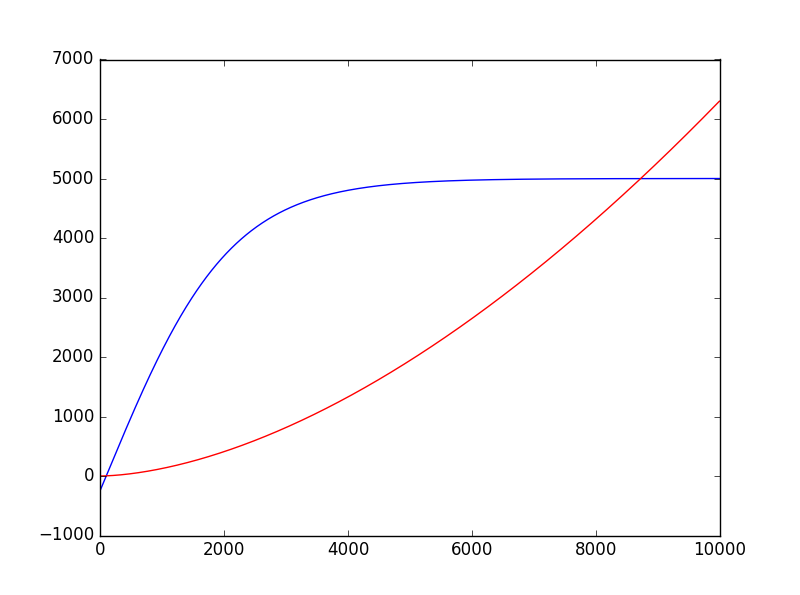
\includegraphics[width=4cm, height=5cm]{figure_1}
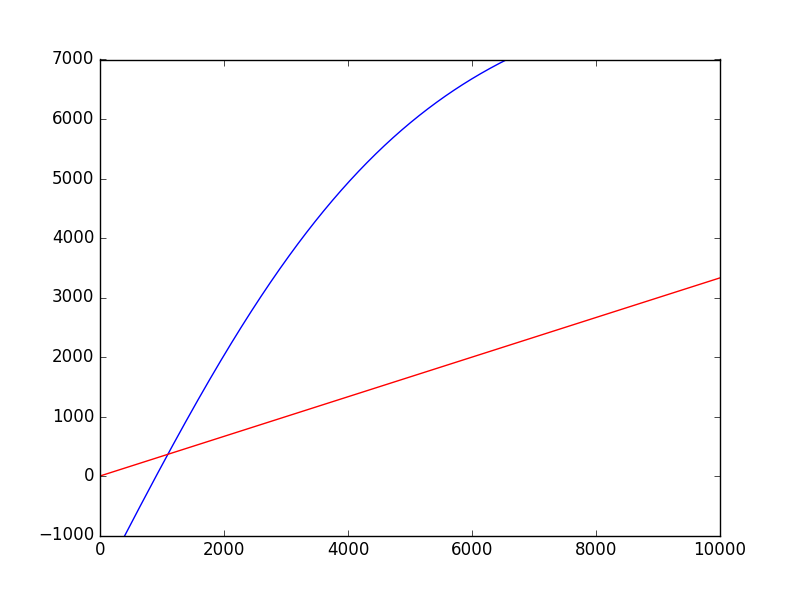
\includegraphics[width=4cm, height=5cm]{figure_2}
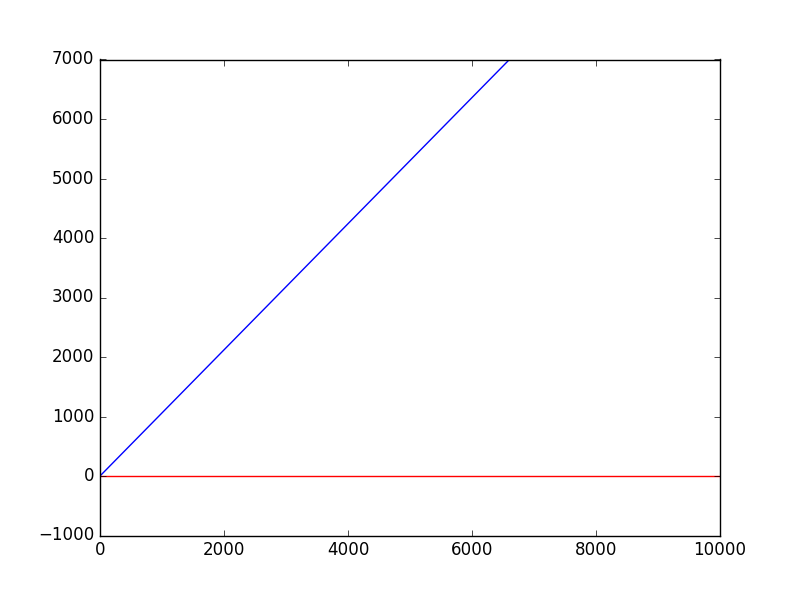
\includegraphics[width=4cm, height=5cm]{figure_3}



Suppose our investor wants to maximize possible return while keeping variance under 1500.
Calling $$V(10000, 3, 1500)$$ would output $$[1800, 4730, 3470]$$ which means our investor would want to invest 1800 in project 1, 4730 in project 2, and 3470 in project 3. 
\newline The total return would be $$\mu_{1}(1800) + \mu_{2}(4730) + \mu_{3}(3470) = 12745.20 $$ and the total variance would be $$\sigma_{1}(1800) + \sigma_{2}(4730) + \sigma_{3}(3470) = 1497.46 \leq 1500 \hspace{.5cm} \checkmark$$
\newline
Or, suppose our investor is much more conservative, and wants to keep variance under 500.  Calling $$V(10000, 3, 500)$$ would output $$[1300, 7790, 910]$$. 
\newline The total return would be $$\mu_{1}(1300) + \mu_{2}(7790) + \mu_{3}(910) = 10948.62 $$ and the total variance would be $$\sigma_{1}(1300) + \sigma_{2}(7790) + \sigma_{3}(910) = 499.68 \leq 1500 \hspace{.5cm} \checkmark$$
\newline
If our investor doesn't care about risk at all, and simply wants to maximize expected return no matter what, they can pass in infinity, or maxint as the third parameter.  The Python call would look like $$V(10000, 3, float('inf'))$$ and would output $$[2090, 3610, 4300]$$. This is essentially the same problem as the general problem we considered in the previous problem.  
The total return would be $$\mu_{1}(2090) + \mu_{2}(3610) + \mu_{3}(4300) = 12882.12 $$ and the total variance would be $$\sigma_{1}(2090) + \sigma_{2}(3610) + \sigma_{3}(4300) = 1872.71 $$
Here are the graphs of our return and variance functions, this time with the computed points overlaid on them.  The green represents a risk tolerance of 1500, the purple represents a risk tolerance of 500 and the black represents an infinite risk tolerance.
\newline

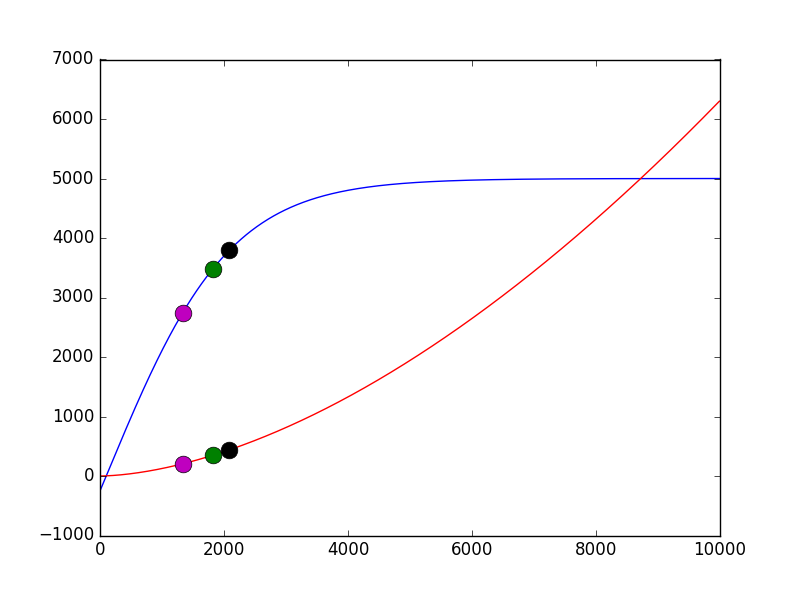
\includegraphics[width=4cm, height=5cm]{data_1}
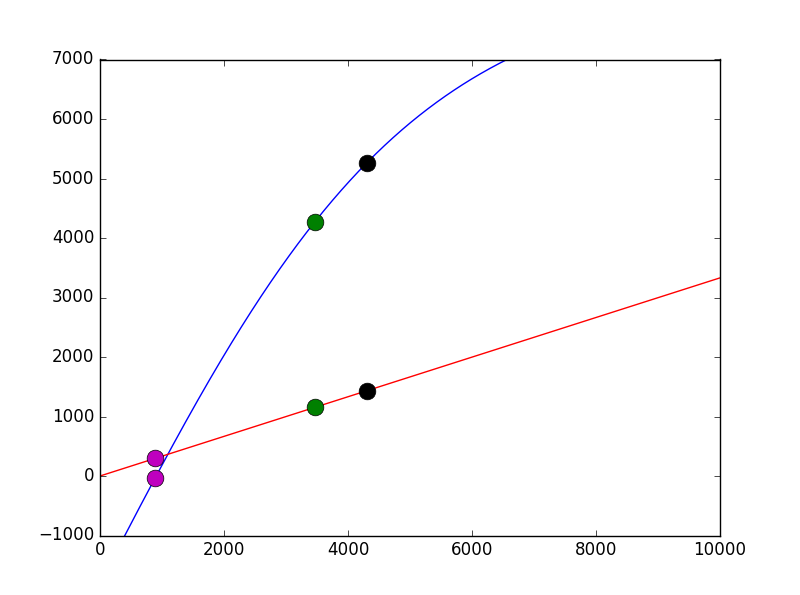
\includegraphics[width=4cm, height=5cm]{data_2}
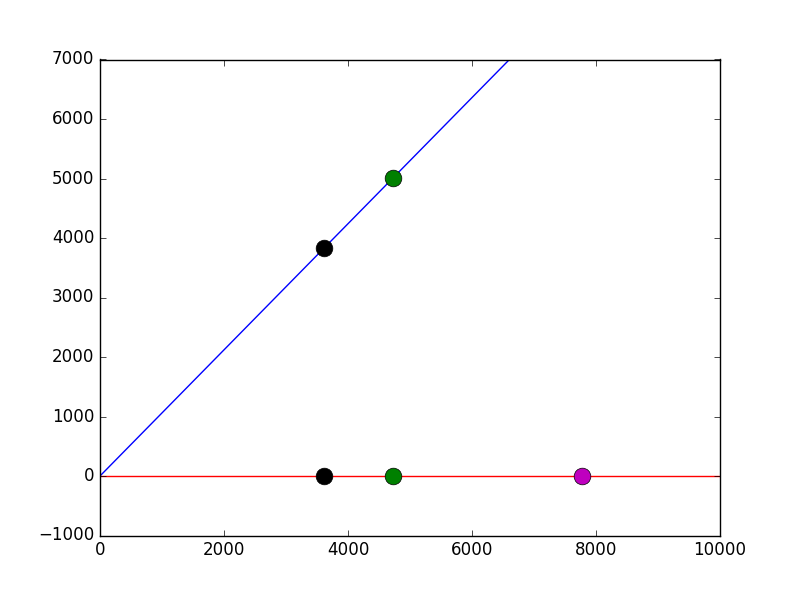
\includegraphics[width=4cm, height=5cm]{data_3}


\newline
\pagebreak
\section{Analysis}
The solution to the general problem benefited greatly by using a dynamic programming solution.  Using a cache to not have to redo computations effectively reduced the runtime from $$O(n^{m})$$ to $$O(n*m)$$ where n is the number of investment projects, and m is the amount to invest.  This reduction in worst case behavior is due to the fact that we are never going to have to recompute a sub problem more than once.  
\newline
With the problem that we have presented an algorithm for, the problem where our returns are given by a stochastic process, we don't see the same improvement.  The runtime of this problem, without dynamic programming is $$O(n^{m})$$ again since in the worst case, we would have to compute each sub problem exactly once. With our dynamic programming algorithm that we presented in the previous section, we don't see an improvement in worst case runtime; the runtimes is still $$O(n^{m})$$. This is largely due to the fact that our cache is now storing values in terms of three variables and we are no longer guaranteed any cache hits at all. 

\newline
It can be shown that $$V(j, x, s1)$$ is not necessarily equal to $$V(j, x, s2)$$ for $$s1 != s2$$.
\newline
Since we are not iterating over the entire range of $$\mu_{n}(m),$$ we are not guaranteed that that final $s$ term will have ever been seen before.  This means that we are not guaranteed any cache hits. And because of this, in the worst case, we will not have any cache hits at all and our runtime will still be $n^{m}$. In the worst case, there is only one possible solution which satisfies the risk requirement, and it happens to be the last one, so all possible solutions must be checked to determine it.  
\newline
This is not to say that caching the results to previous subproblems is all bad.  In fact, we have found that it actually reduces the average runtime significantly in many cases. However, not by an order of magnitude, since the cache hits are much more infrequent.  We've also found that a higher correlation between the variance and expected return functions produces more cache hits, as do linear variance functions. In summary, the number of cache hits for our algorithm is not guaranteed, and is highly dependent on the inputs.  
\par 
It appears that this problem may actually be NP-Hard, as we cannot solve it in polynomial time, and we can't verify it in polynomial time either.  In order to verify that a solution is correct, we have to check that it does in fact give a greater expected return than all other possible solutions, and in order to do this we need to solve for all other possible solutions.  
\pagebreak
\begin{thebibliography}{9}


\bibitem{Ross} 
Sheldon M. Ross 
\textit{An Elementary Introduction To Mathematical Finance}. 
Cambridge University Press, New York, NY, 1999.
 


\end{document}
